% !TEX root = ../../manuscript-SI.tex

\section{Computational details}\label{si-computational-details}

\subsection{Force field parameters for D4}\label{force-field-parameters-for-d4}

D4 was modelled as a semi-flexible molecule with an all atom atomistic model.
All intramolecular bonds, angles, dihedrals, and cross terms parameters for
methyl groups were taken from the consistent-valence force field (CVFF).
\citep{dauber-osguthorpeStructureEnergeticsLigand1988}

\textbf{Harmonic Bond}

\begin{equation}
    U = \frac{1}{2}p_{0}{(r - p_{1})}^{2}
\end{equation}

where \(p_0 / \kappa_B\) in units K/Ų, \(p_{1}\) in Å. 

\begin{table}[H]
    \centering
    \caption{%
        D4 bonding potential parameters.
    }\label{tbl:ff-d4-bond}
    \begin{tabular}{@{}llll@{}}
        Pseudo atom & Type of bond & \(p_0 / \kappa_B\) (K/Ų) & \(p_{1}\) (Å) \\
        \midrule
        Si-O & RIGID\_BOND & - & -\\
        Si-C & HARMONIC\_BOND & 286248.126 & 1.809\\
        C3-H & HARMONIC\_BOND & 409668.576 & 1.105\\
        \bottomrule
    \end{tabular}
\end{table}

\textbf{Harmonic Bend}

\begin{equation}
    U = \frac{1}{2}p_{0}{(\theta_{\text{ijk}} - p_{1})}^{2}
\end{equation}

where \(p_0 / \kappa_B\) in units K/rad², \(p_{1}\) in degree.

\begin{table}[H]
    \centering
    \caption{%
        D4 bending potential parameters.
    }\label{tbl:ff-d4-bend}
    \begin{tabular}{@{}llll@{}}
        Pseudo atom & Type of angle & \(p_0 / \kappa_B\) (K/rad²) & \(p_1\) (°) \\
        \midrule
        Si-C-H & HARMONIC\_BEND & 41614.223 & 112.3\\
        C-Si-C & HARMONIC\_BEND & 53400.911 & 113.5\\
        C-Si-O & HARMONIC\_BEND & 53040.094 & 117.3\\
        H-C-H & HARMONIC\_BEND & 47507.567 & 106.4\\
        \bottomrule
    \end{tabular}
\end{table}

\textbf{CVFF Dihedral}

\begin{equation}
    U = p_{0}{(1 + cos(p_{1}\phi_{\text{ijk}} - p_{2}))}^{2}
\end{equation}

where \(p_0 / \kappa_B\) in units K, \(p_2\) in degree. 

\begin{table}[H]
    \centering
    \caption{%
        D4 dihedral potential parameters.
    }\label{tbl:ff-d4-dihedral}
    \begin{tabular}{@{}lllll@{}}
        Pseudo atom & Type of torsion & \(p_0 / \kappa_B\) (K) & \(p_1\) (multiplicity) & \(p_2\) (°) \\
        \midrule
        H-C-Si-C & CVFF\_DIHEDRAL & 240.545 & 3 & 0\\
        H-C-Si-O & CVFF\_DIHEDRAL & -60.136 & 3 & 0\\
        C-Si-O-Si & CVFF\_DIHEDRAL & 240.545 & 3 & 0\\
        \bottomrule
    \end{tabular}
\end{table}

\textbf{CFF Bond Bond Cross}

\begin{equation}
    U = p_{0}(r - p_{1})(r\prime - p_{2})
\end{equation}

where \(p_0 / \kappa_B\) in units K/Ų, \(p_1\) and \(p_2\) in Å

\begin{table}[H]
    \centering
    \caption{%
        D4 cross-term bonding potential parameters.
    }\label{tbl:ff-d4-cross-bond}
    \begin{tabular}{@{}lllll@{}}
        Pseudo atom & Type of bond-bond & \(p_0 / \kappa_B\) (K/Ų) & \(p_1\) (Å) & \(p_2\) (Å) \\
        \midrule
        Si-C-H & CFF\_BOND\_BOND\_CROSS & 14312.406 & 0 & 0\\
        C-Si-C & CFF\_BOND\_BOND\_CROSS & 7336.612 & 0 & 0\\
        C-Si-O & CFF\_BOND\_BOND\_CROSS & 25257.188 & 0 & 0\\
        \bottomrule
    \end{tabular}
\end{table}

\pagebreak

\textbf{CFF Bond Bend Cross}

\begin{equation}
    U = {(\theta - p}_{0}) [p_{1}(r - p_{2}) + p_{3}(r\prime - p_{4})]
\end{equation}

where \(p_0\) in degrees, \(p_1\) and \(p_3\) in units K/Å/rad, \(p_1\) and \(p_2\) in Å.

\begin{table}[H]
    \centering
    \caption{%
        D4 cross-term bonding-bending potential parameters.
    }\label{tbl:ff-d4-cross-bondbend}
    \begin{tabular}{@{}lllllll@{}}
        Pseudo atom & Type of bond-angle & po (°) & \(p_1\) (K/Å/rad) & \(p_2\) (Å) & \(p_3\) (K/Å/rad) & \(p_4\) (Å) \\
        \midrule
        Si-C-H & CFF\_BOND\_BEND\_CROSS & 0 & 14733.359 & 0 & 9742.06 & 0\\
        C-Si-C & CFF\_BOND\_BEND\_CROSS & 0 & 781.770 & 0 & 0 & 0\\
        C-Si-O & CFF\_BOND\_BEND\_CROSS & 0 & 11425.871 & 0 & 27061.27 & 0\\
        \bottomrule
    \end{tabular}
\end{table}

\textbf{D4 LJ parameters and charges}

The electronic potential (ESP) derived partial charges of D4 were computed by
density functional theory (DFT) calculations with PBE (Perdew-Burke-Ernzerhof)
functional \citep{perdewGeneralizedGradientApproximation1996} and DNP (double
numeric plus polarization) basis set
\citep{hehreSelfconsistentMolecularOrbital1972}, using DMol\textsuperscript{3}
module \citep{delleyAllElectronNumerical1990} in Materials Studio
\citep{accelrysMaterialsStudio2001} (\cref{tbl:ff-d4-charge}).

\begin{table}[H]
    \centering
    \caption{%
        Charges and Lennard-Jones parameters for all atoms of D4.
    }\label{tbl:ff-d4-charge}
    \begin{tabular}{@{}llll@{}}
        Pseudo atom & Charge (e\textsuperscript{-}) & \(\epsilon / \kappa_B\) (K) & \(\sigma\) (Å) \\
        \midrule
        Si & 1.321 & 202.429 & 3.826\\
        O & -0.763 & 30.213 & 3.118\\
        C & -0.889 & 52.873 & 3.431\\
        H & 0.2032 & 22.156 & 2.571\\
        \bottomrule
    \end{tabular}
\end{table}


\subsection{Screening dataset}\label{si-screening-dataset}

1710 non-disordered MOFs with pore limiting diameters \textgreater{} 6 Å were
screened from CoRE-MOF database, to which 29 well-known MOFs were added with
proven stability and high porosity, including the MOF-74 isoreticular series
\citep{gulcayBiocompatibleMOFsStorage2019}, Cr-soc-MOF-1
\citep{nandiRevisitingWaterSorption2019}, UiO-68 (UiO for University of Oslo),
MOF-808, \citep{soaresComputationalEvaluationChemical2019} and a several
structures originating from Dresden University of Technology (DUT) and Material
of Institute Lavoisier (MIL). This additional list is given in \cref{tbl:extra-mofs}.

The combined dataset of 1739 MOFs show a broad range of geometric and textural
features: PLDs (6.0--71.5 Å), \ce{N2} accessible SA
(320--\SI{6770}{\metre\squared\per\gram}), density (0.13--2.22
\si{\gram\per\centi\metre\cubed}), \(\phi\) (0.42--0.94) and PVs (0.23--7.46
\si{\centi\metre\cubed\per\gram}).

\begin{table}[H]
    \centering
    \caption{%
        Details of the 29 MOFs added to the COREMOF database.
    }\label{tbl:extra-mofs}
    \begin{tabular}{@{}llll@{}}
        MOFs & Reference & MOFs & Reference\\
        \midrule
        RAVWAO & \citep{gulcayBiocompatibleMOFsStorage2019} & 
        DUT-5 & \citep{senkovskaNewHighlyPorous2009} \\
        RAVWES & \citep{gulcayBiocompatibleMOFsStorage2019} &
        DUT-51-Zr & \citep{bonZrIvHf2012}\\
        RAVWIW & \citep{gulcayBiocompatibleMOFsStorage2019} &
        DUT-67-Zr & \citep{bonZrHfBasedMetal2013}\\
        RAVWOC & \citep{gulcayBiocompatibleMOFsStorage2019} &
        MIL-68(Al) & \citep{yangProbingAdsorptionPerformance2012}\\
        RAVWUI & \citep{gulcayBiocompatibleMOFsStorage2019} &
        Cr-soc-MOF-1 & \citep{nandiRevisitingWaterSorption2019}\\
        RAVXAP & \citep{gulcayBiocompatibleMOFsStorage2019} &
        MIP\textsuperscript{{[}4{]}}-177 & \citep{wangPhaseTransformableUltrastable2018} \\
        RAVXET & \citep{gulcayBiocompatibleMOFsStorage2019} &
        MIP-200 & \citep{wangRobustLargeporeZirconium2018} \\
        RAVXIX & \citep{gulcayBiocompatibleMOFsStorage2019} &
        Zr-IPA\textsuperscript{{[}5{]}} & \citep{wangMesoporousZirconiumIsophthalateMultifunctional2020} \\
        MIL-125 & \citep{soaresComputationalEvaluationChemical2019} &
        Ni-BPM\textsuperscript{{[}6{]}} & \citep{zhengMolecularInsightFluorocarbon2020}\\
        MOF-808-acetate & \citep{soaresComputationalEvaluationChemical2019} &
        Ni-BPP\textsuperscript{{[}7{]}} & \citep{zhengMolecularInsightFluorocarbon2020}\\
        MOF-808-formate & \citep{soaresComputationalEvaluationChemical2019} &
        Ni-TPM\textsuperscript{{[}8{]}} & \citep{zhengMolecularInsightFluorocarbon2020}\\
        NU\textsuperscript{{[}1{]}}-1000 & \citep{soaresComputationalEvaluationChemical2019} &
        Ni-TPP\textsuperscript{{[}9{]}} & \citep{zhengMolecularInsightFluorocarbon2020}\\
        UiO\textsuperscript{{[}2{]}}-68 & \citep{soaresComputationalEvaluationChemical2019} &
        Ni-MOF-74 & \citep{zhengMolecularInsightFluorocarbon2020}\\
        Zr6-AzoBDC\textsuperscript{{[}3{]}} & \citep{soaresComputationalEvaluationChemical2019} &
        PCN\textsuperscript{{[}10{]}}-224(Ni) & \citep{fengConstructionUltrastablePorphyrin2013}\\
        \bottomrule
        \multicolumn{4}{l}{{[}1{]}NU: Northwestern University; {[}2{]}UiO: University of Oslo;}\\
        \multicolumn{4}{l}{{[}3{]}AzoBDC: azobenzenedicarboxylate;}\\
        \multicolumn{4}{l}{{[}4{]}MIP: material of the Institute of Porous Materials from Paris;}\\
        \multicolumn{4}{l}{{[}5{]}IPA: isophatale; {[}6{]}BPM: biphenyl-meta;}\\
        \multicolumn{4}{l}{{[}7{]}BPP: biphenyl-para; {[}8{]}TPM: triphenyl-meta;}\\
        \multicolumn{4}{l}{{[}9{]}TPP: triphenyl-para; {[}10{]}PCN: Porous coordination network;}\\
    \end{tabular}
\end{table}

\begin{figure}[H]
    \centering
    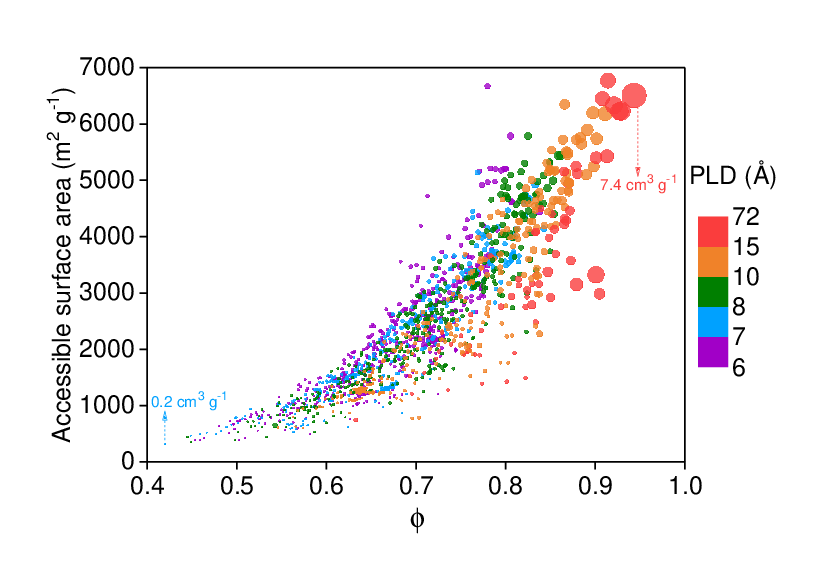
\includegraphics[width=0.8\textwidth]{dataset_geometric}
    \caption{%
        Overview of the diversity of the MOF database with
        PLD > 6 Å in terms of void fractions, accessible surface
        areas and PLDs. Data points are color coded by PLDs of MOFs. Pore
        volumes of all structures are represented by size.
    }\label{fig:d4-screening-geometric}
\end{figure}

\begin{figure}[H]
    \centering
    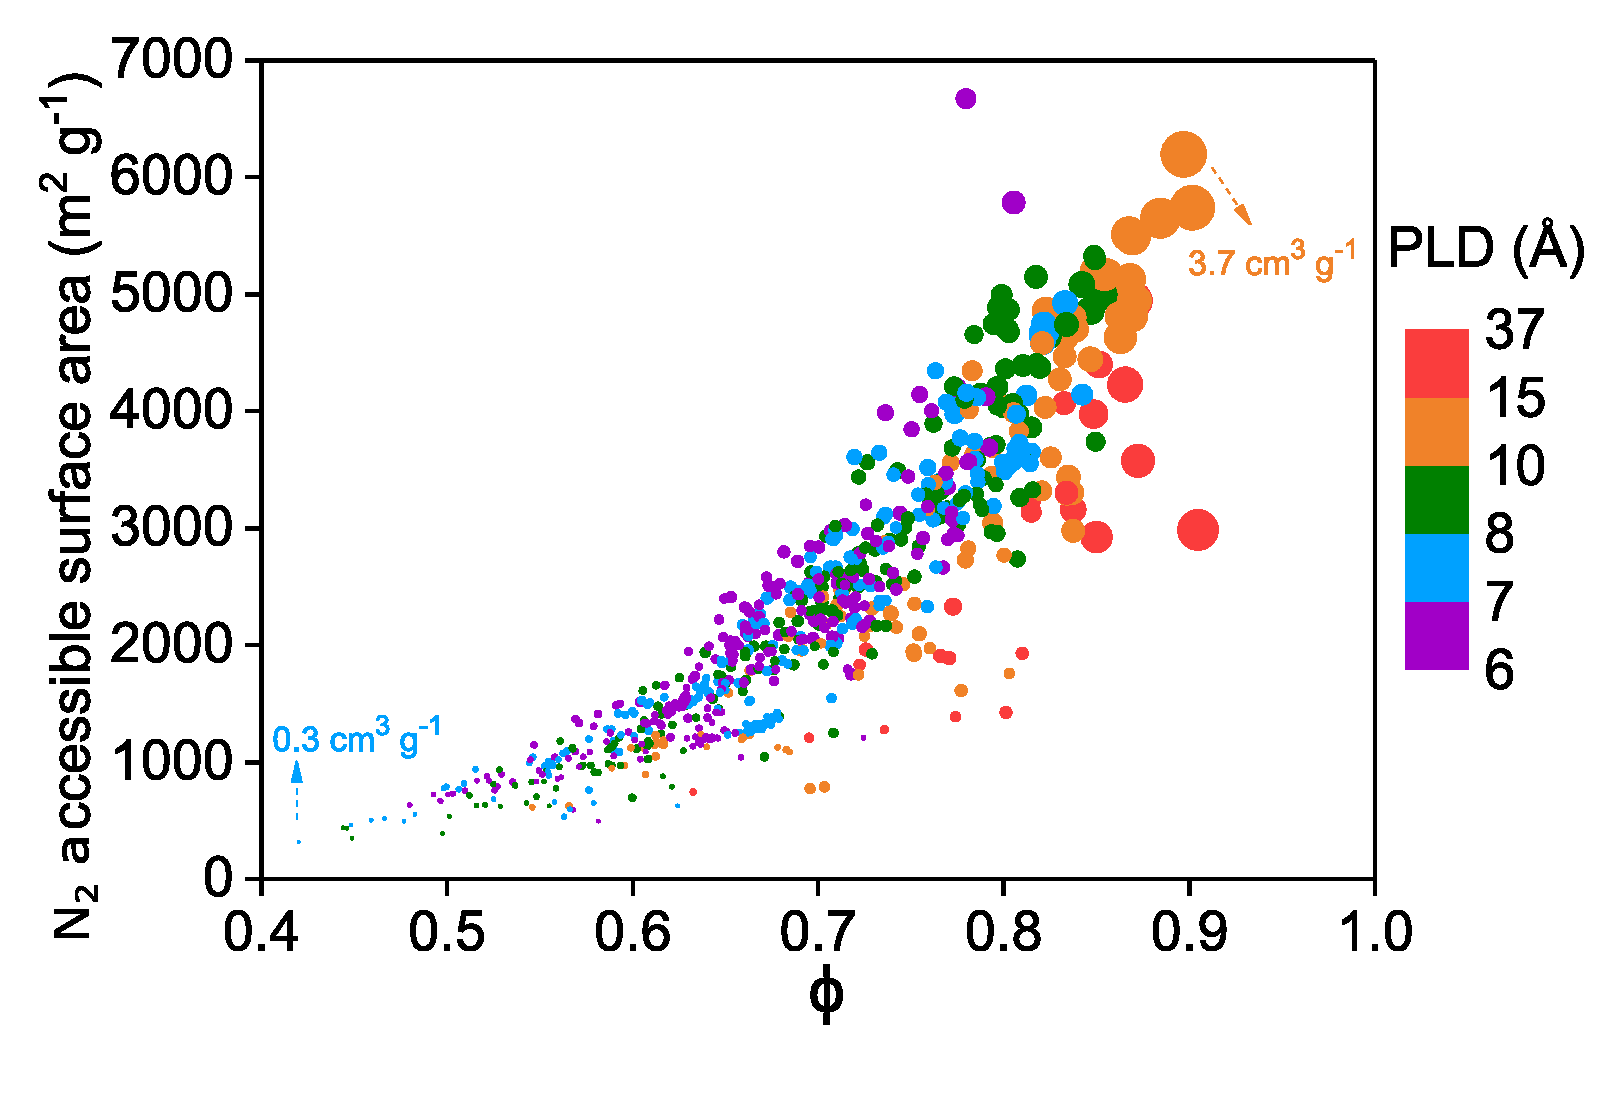
\includegraphics[width=0.8\textwidth]{dataset_hydrophobic}
    \caption{%
        Overview of the diversity of the hydrophobic MOFs
        database in terms of void fraction and accessible surface areas. Data
        points are color coded by PLDs of MOFs. Pore volumes of all structures
        are represented by size.
    }\label{fig:d4-screening-hydrophobic}
\end{figure}

\begin{figure}[H]
    \centering
    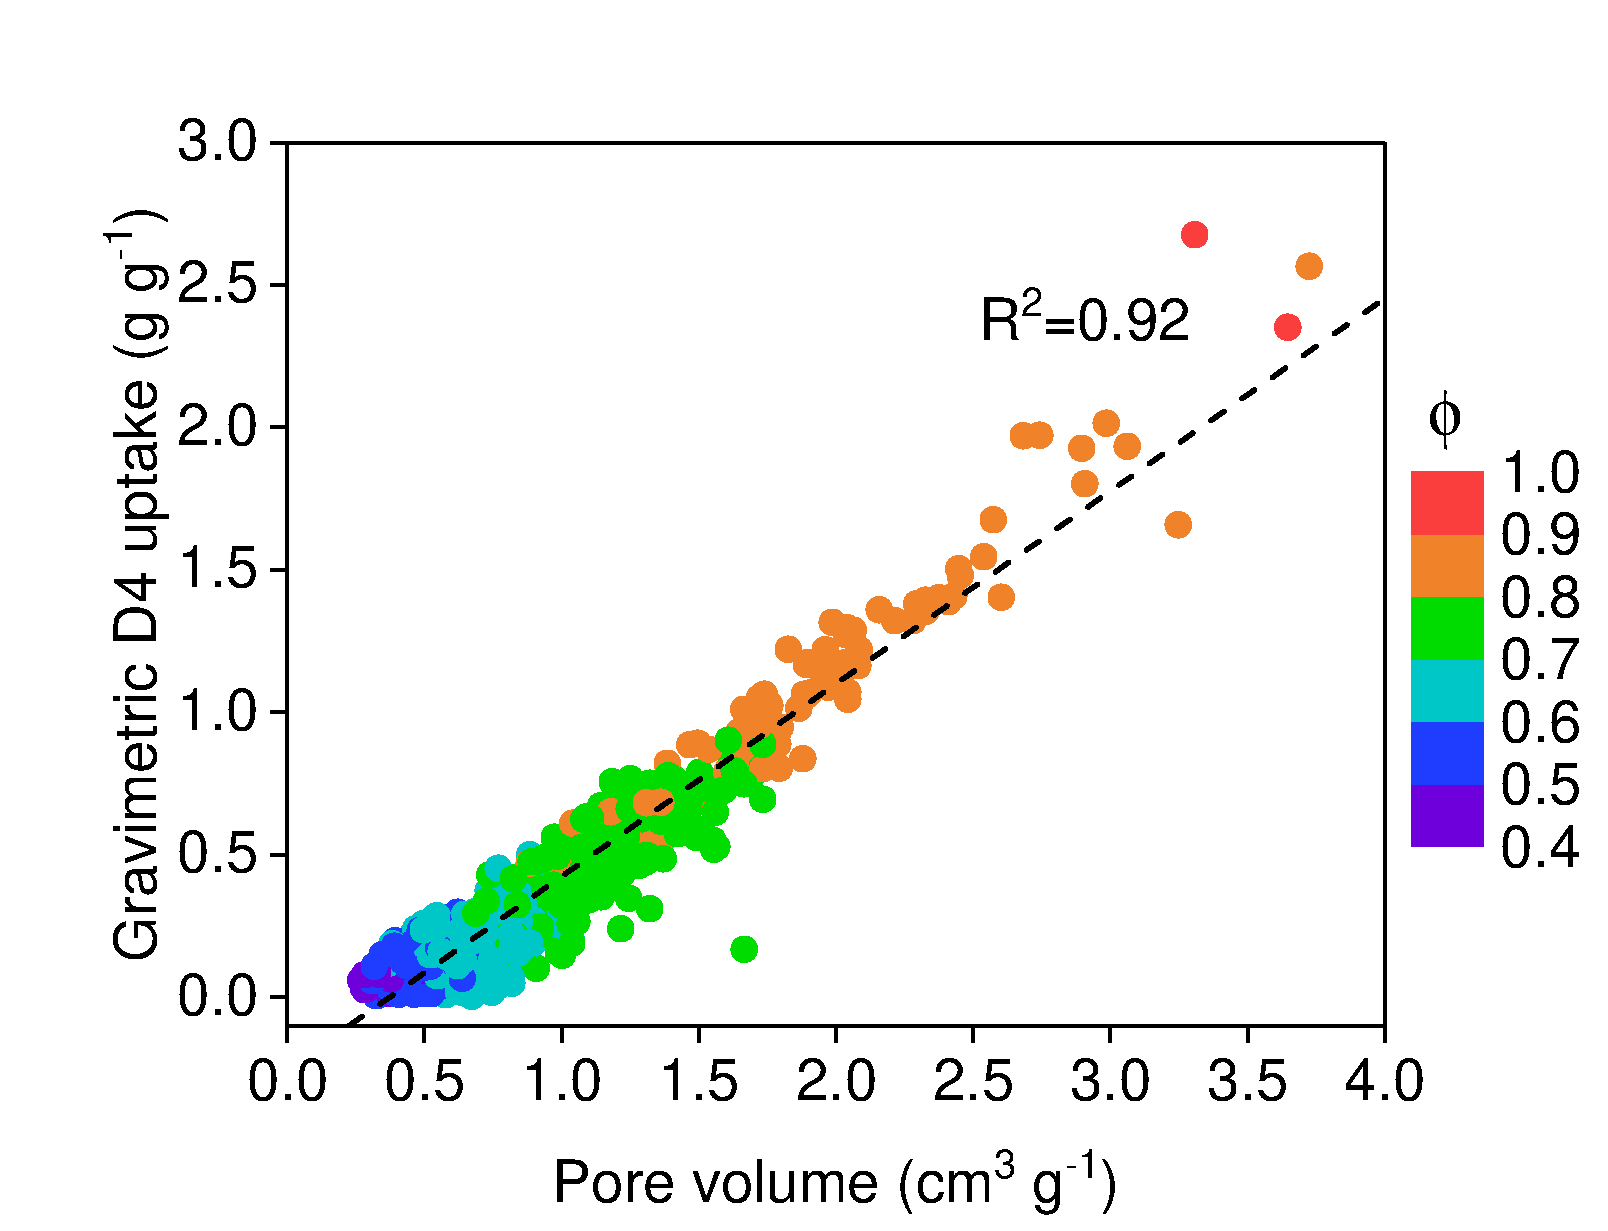
\includegraphics[width=0.8\textwidth]{dataset_gv}
    \caption{%
        The relation of gravimetric D4 uptake of the 811 hydrophobic MOFs
        (g g\textsuperscript{-1}) and their pore volumes
        (cm\textsuperscript{3} g\textsuperscript{-1}), color coded by void fraction of the
        MOFs.
    }\label{fig:d4-screening-grav-volum}
\end{figure}

\begin{figure}[H]
    \centering
    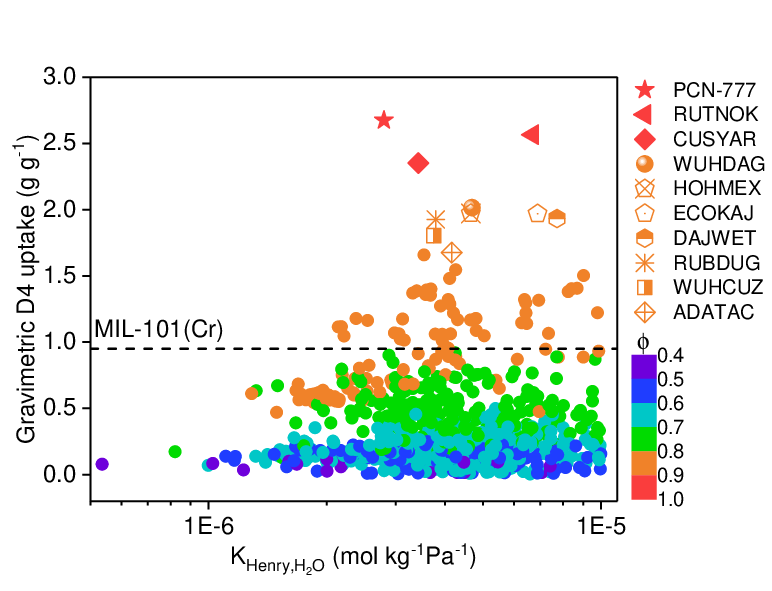
\includegraphics[width=0.8\textwidth]{dataset_kh}
    \caption{%
        Predicted D4 uptake performance at 298 K for the hydrophobic MOFs
        database plotted as a function of their computed Henry constant for
        water, color coded by void fraction, \(\phi\). Top performing 10
        candidates are represented by different symbols in the legend to the
        right.
    }\label{fig:d4-screening-henryc}
\end{figure}

\pagebreak

{\footnotesize
\begin{longtable}[]{@{}p{5cm}p{12cm}@{}}
    \caption{Structural details of the top promising 10 hydrophobic materials which exhibit the highest D4 uptake.}\label{tbl:top-mofs-detail}\\
    \toprule
    \thead{MOF} & \thead{Details} \\
    \midrule
    \makecell{\textbf{FOTNIN (PCN-777)} \\ 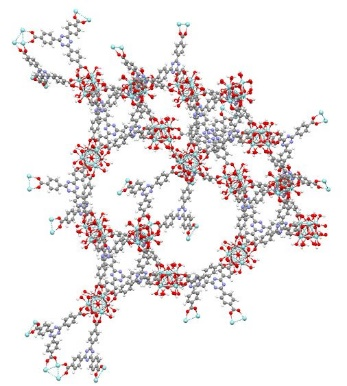
\includegraphics[height=3cm]{top10/image6.jpeg}}
    & \makecell[l]{
        \textbf{Organic ligand:} 4,4`,4`-s-triazine-2,4,6-triyl-tribenoic acid \\
        \textbf{Metal site:} Zr \\
        \textbf{PLD:} 28.36 Å \\
        \textbf{SA:} \SI{2990}{\metre\squared\per\gram} \\
        \textbf{Density:} \SI{0.27}{\gram\per\centi\metre\cubed} \\
        \textbf{PV:} \SI{3.31}{\centi\metre\cubed\per\gram} \\
        \textbf{\(\phi\):} 0.90 \\
        \textbf{Gravimetric D4 uptake:} \SI{2.68}{\gram\per\gram} \\
        \textbf{Volumetric D4 uptake:} \SI{0.72}{\gram\per\centi\metre\cubed}}\\
    \midrule
    \makecell{\textbf{RUTNOK (IRMOF-76)} \\ 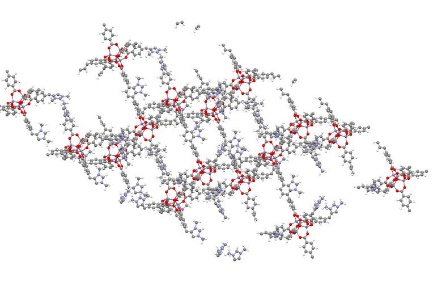
\includegraphics[height=3cm]{top10/image7.jpeg}}
    & \makecell[l]{
        \textbf{Organic ligand:} \\
        4,7-bis(4-carboxylphenyl)-1,3-dimethylbenzimidazium-tetrafluoroborate \\
        \textbf{Metal site:} Zn \\
        \textbf{PLD:} 14.65 Å \\
        \textbf{SA:} \SI{6200}{\metre\squared\per\gram} \\
        \textbf{Density:} \SI{0.24}{\gram\per\centi\metre\cubed} \\
        \textbf{PV:} \SI{3.72}{\centi\metre\cubed\per\gram} \\
        \textbf{\(\phi\):} 0.90 \\
        \textbf{Gravimetric D4 uptake:} \SI{2.57}{\gram\per\gram} \\
        \textbf{Volumetric D4 uptake:} \SI{0.62}{\gram\per\centi\metre\cubed}}\\
    \midrule
    \makecell{\textbf{CUSYAR (MOF-210)} \\ 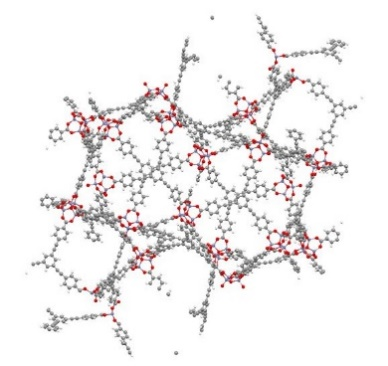
\includegraphics[height=3cm]{top10/image8.jpeg}}
    & \makecell[l]{
        \textbf{Organic ligand:} biphenyl-4,4'-dicarboxylate \\
        \textbf{Metal site:} Zn \\
        \textbf{PLD:} 12.18 Å \\
        \textbf{SA:} \SI{5700}{\metre\squared\per\gram} \\
        \textbf{Density:} \SI{0.25}{\gram\per\centi\metre\cubed} \\
        \textbf{PV:} \SI{3.65}{\centi\metre\cubed\per\gram} \\
        \textbf{\(\phi\):} 0.90 \\
        \textbf{Gravimetric D4 uptake:} \SI{2.35}{\gram\per\gram} \\
        \textbf{Volumetric D4 uptake:} \SI{0.59}{\gram\per\centi\metre\cubed}}\\
    \midrule
    \makecell{\textbf{WUHDAG (NU-1104)} \\ 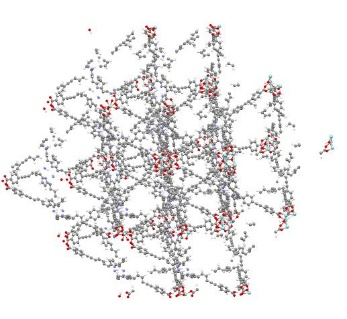
\includegraphics[height=3cm]{top10/image9.jpeg}}
    & \makecell[l]{
        \textbf{Organic ligand:} meso-tetrakis-(4-((phenyl)ethynyl)benzoate) porphyrin \\
        \textbf{Metal site:} Zr \\
        \textbf{PLD:} 10.50 Å \\
        \textbf{SA:} \SI{5500}{\metre\squared\per\gram} \\
        \textbf{Density:} \SI{0.29}{\gram\per\centi\metre\cubed} \\
        \textbf{PV:} \SI{2.99}{\centi\metre\cubed\per\gram} \\
        \textbf{\(\phi\):} 0.87 \\
        \textbf{Gravimetric D4 uptake:} \SI{2.01}{\gram\per\gram} \\
        \textbf{Volumetric D4 uptake:} \SI{0.58}{\gram\per\centi\metre\cubed}}\\
    \midrule
    \makecell{\textbf{HOHMEX} \\ 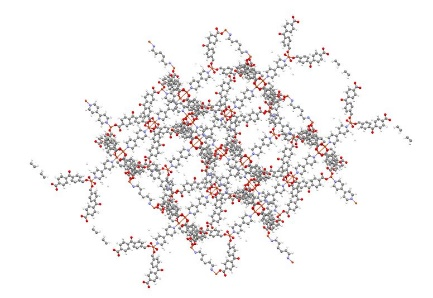
\includegraphics[height=3cm]{top10/image10.jpeg}}
    & \makecell[l]{
        \textbf{Organic ligand:} 4,4'-carbonyldibenzoato - (\(\mu\)2-4,4'-bipyridine) \\
        \textbf{Metal site:} Cu \\
        \textbf{PLD:} 14.89 Å \\
        \textbf{SA:} \SI{5000}{\metre\squared\per\gram} \\
        \textbf{Density:} \SI{0.32}{\gram\per\centi\metre\cubed} \\
        \textbf{PV:} \SI{2.74}{\centi\metre\cubed\per\gram} \\
        \textbf{\(\phi\):} 0.87 \\
        \textbf{Gravimetric D4 uptake:} \SI{1.97}{\gram\per\gram} \\
        \textbf{Volumetric D4 uptake:} \SI{0.63}{\gram\per\centi\metre\cubed}}\\
    \midrule
    \makecell{\textbf{ECOKAJ} \\ 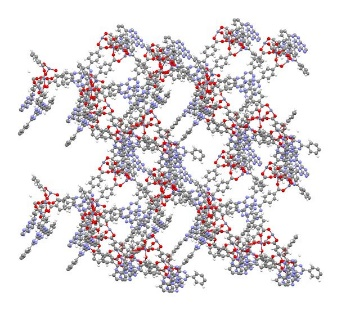
\includegraphics[height=3cm]{top10/image11.jpeg}}
    & \makecell[l]{
        \textbf{Organic ligand:} s-heptazine tribenzoate \\
        \textbf{Metal site:} Zn \\
        \textbf{PLD:} 17.58 Å \\
        \textbf{SA:} \SI{3600}{\metre\squared\per\gram} \\
        \textbf{Density:} \SI{0.33}{\gram\per\centi\metre\cubed} \\
        \textbf{PV:} \SI{2.68}{\centi\metre\cubed\per\gram} \\
        \textbf{\(\phi\):} 0.87 \\
        \textbf{Gravimetric D4 uptake:} \SI{1.97}{\gram\per\gram} \\
        \textbf{Volumetric D4 uptake:} \SI{0.65}{\gram\per\centi\metre\cubed}}\\
    \midrule
    \makecell{\textbf{DAJWET} \\ 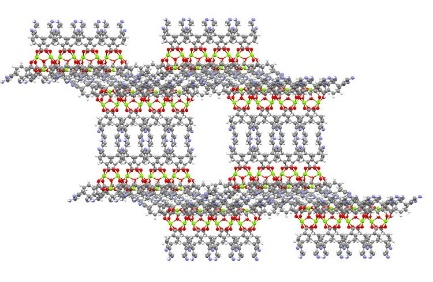
\includegraphics[height=3cm]{top10/image12.jpeg}}
    & \makecell[l]{
        \textbf{Organic ligand:} tetrakis (4-carboxylatophenyl) porphyrin \\
        \textbf{Metal site:} Mg \\
        \textbf{PLD:} 26.59 Å \\
        \textbf{SA:} \SI{5000}{\metre\squared\per\gram} \\
        \textbf{Density:} \SI{0.28}{\gram\per\centi\metre\cubed} \\
        \textbf{PV:} \SI{3.06}{\centi\metre\cubed\per\gram} \\
        \textbf{\(\phi\):} 0.87 \\
        \textbf{Gravimetric D4 uptake:} \SI{1.93}{\gram\per\gram} \\
        \textbf{Volumetric D4 uptake:} \SI{0.54}{\gram\per\centi\metre\cubed}}\\
    \midrule
    \makecell{\textbf{RUBDUP} \\ 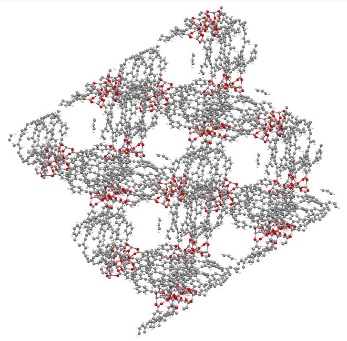
\includegraphics[height=3cm]{top10/image13.jpeg}}
    & \makecell[l]{
        \textbf{Organic ligand:} phenylene ethynylene macrocycle \\
        \textbf{Metal site:} Zn \\
        \textbf{PLD:} 19.25 Å \\
        \textbf{SA:} \SI{4200}{\metre\squared\per\gram} \\
        \textbf{Density:} \SI{0.30}{\gram\per\centi\metre\cubed} \\
        \textbf{PV:} \SI{2.90}{\centi\metre\cubed\per\gram} \\
        \textbf{\(\phi\):} 0.87 \\
        \textbf{Gravimetric D4 uptake:} \SI{1.93}{\gram\per\gram} \\
        \textbf{Volumetric D4 uptake:} \SI{0.58}{\gram\per\centi\metre\cubed}}\\
    \midrule
    \makecell{\textbf{WUHCUZ (NU-1103)} \\ 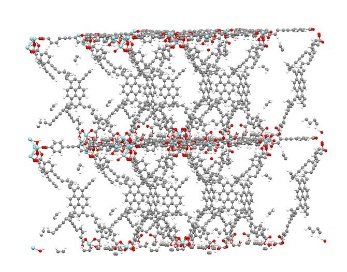
\includegraphics[height=3cm]{top10/image14.jpeg}}
    & \makecell[l]{
        \textbf{Organic ligand:} \\
        {\tiny 4,4`,4``,4```-((pyrene-1,3,6,8 tetrayltetrakis(benzene-4,1-diyl)) tetrakis(ethyne-2,1 diyl))tetrabenzoate} \\
        \textbf{Metal site:} Zr \\
        \textbf{PLD:} 12.21 Å \\
        \textbf{SA:} \SI{5500}{\metre\squared\per\gram} \\
        \textbf{Density:} \SI{0.30}{\gram\per\centi\metre\cubed} \\
        \textbf{PV:} \SI{2.91}{\centi\metre\cubed\per\gram} \\
        \textbf{\(\phi\):} 0.87 \\
        \textbf{Gravimetric D4 uptake:} \SI{1.80}{\gram\per\gram} \\
        \textbf{Volumetric D4 uptake:} \SI{0.54}{\gram\per\centi\metre\cubed}}\\
    \midrule
    \makecell{\textbf{ADATAC} \\ 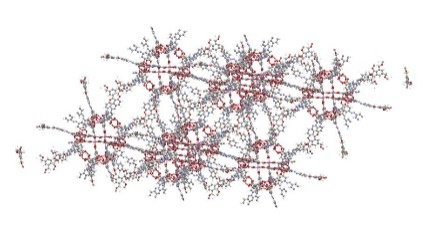
\includegraphics[height=3cm]{top10/image15.jpeg}}
    & \makecell[l]{
        \textbf{Organic ligand:} \\
        5,5`,5``-(4,4`,4``-{[}1,3,5-phenyltris(methoxy){]} tris-phenylazo) tris-isophthalic acid \\
        \textbf{Metal site:} Zn \\
        \textbf{PLD:} 10.28 Å \\
        \textbf{SA:} \SI{5130}{\metre\squared\per\gram} \\
        \textbf{Density:} \SI{0.34}{\gram\per\centi\metre\cubed} \\
        \textbf{PV:} \SI{2.57}{\centi\metre\cubed\per\gram} \\
        \textbf{\(\phi\):} 0.87 \\
        \textbf{Gravimetric D4 uptake:} \SI{1.68}{\gram\per\gram} \\
        \textbf{Volumetric D4 uptake:} \SI{0.57}{\gram\per\centi\metre\cubed}}\\
    \bottomrule
\end{longtable}
}

\subsection{Radial distribution functions for D4-PCN-777}\label{si-radial-distribution}

\begin{figure}[H]
    \centering
    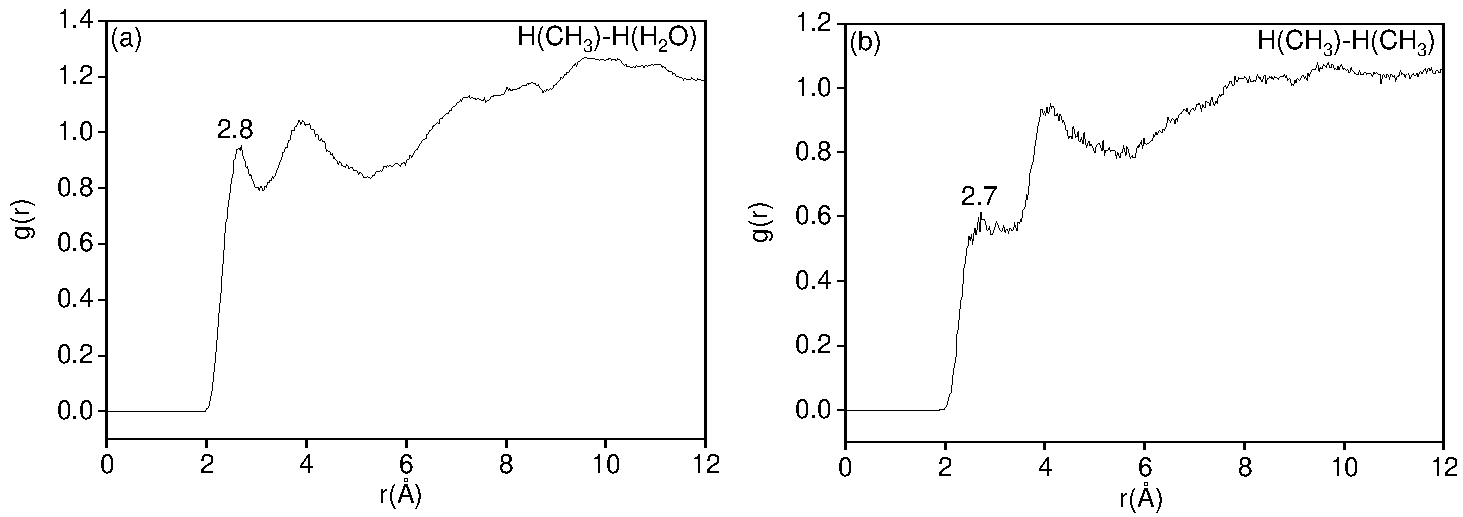
\includegraphics[width=0.9\textwidth]{d4-rdf}
    \caption{%
        All-atom averaged radial distribution functions between (a) H atom from
        \ce{CH3} group of D4 molecules and H atom from coordinated water of the
        framework at 10\% total loading and (b) H atom from \ce{CH3} groups of D4 at
        100\% loading.
    }\label{fig:d4-rdf}
\end{figure}

\pagebreak

\section{MOF samples}\label{mof-samples}

\subsection{MIL-101(Cr)}

The benchmark MIL-101(Cr) sample was taken from a previous work
\citep{pillaiCapturePerformancesHybrid2017}, with all textural characteristics
as stated in reference.

\subsection{DUT-4}

DUT-4 was purchased from Materials Center (TU Dresden, Germany).

\begin{figure}[H]
    \centering
    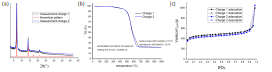
\includegraphics[width=\textwidth]{dut4_summary}
    \caption{%
        Characterization of the DUT-4 sample, in duplicates as black
        and blue: (a) PXRD, alongside simulated pattern in red (b) TGA curves
        and (c) \ce{N2} physisorption isotherms at 77 K.
    }\label{fig:dut4-summary}
\end{figure}

\subsection{PCN-777}

\textbf{Synthesis}

To synthesize the PCN-777, \ce{ZrOCl2*8H2O} (\SI{1.08}{\gram},
\SI{3.351}{\milli\mol}) and 4,4’,4’’-s-Triazine-2,4,6-triyl-tribenzoic acid
(\SI{0.270}{\gram}, \SI{0.612}{\milli\mol}) were put into \SI{36}{\milli\litre}
N,N-Diethylformamide (DEF) in a \SI{100}{\milli\litre} Teflon-lined autoclave
reactor, alongside an amount of trifluoroacetic acid (\SI{1.8}{\milli\litre}) to
form a reaction solution. After sonicating the reaction solution at room
temperature for 10 min, the reactor was transferred to a convection oven
followed by heating at \SI{423}{\kelvin} for 12 h. The PCN-777 crystalline solid
was recovered by filtration after purification with \SI{100}{\milli\litre}
N,N-Dimethylformamide (DMF) and acetone for 3 h at room temperature. The
collected crystalline solid was dried at \SI{393}{\kelvin} for 12 h.

\textbf{Characterisation}

\begin{figure}[H]
    \centering
    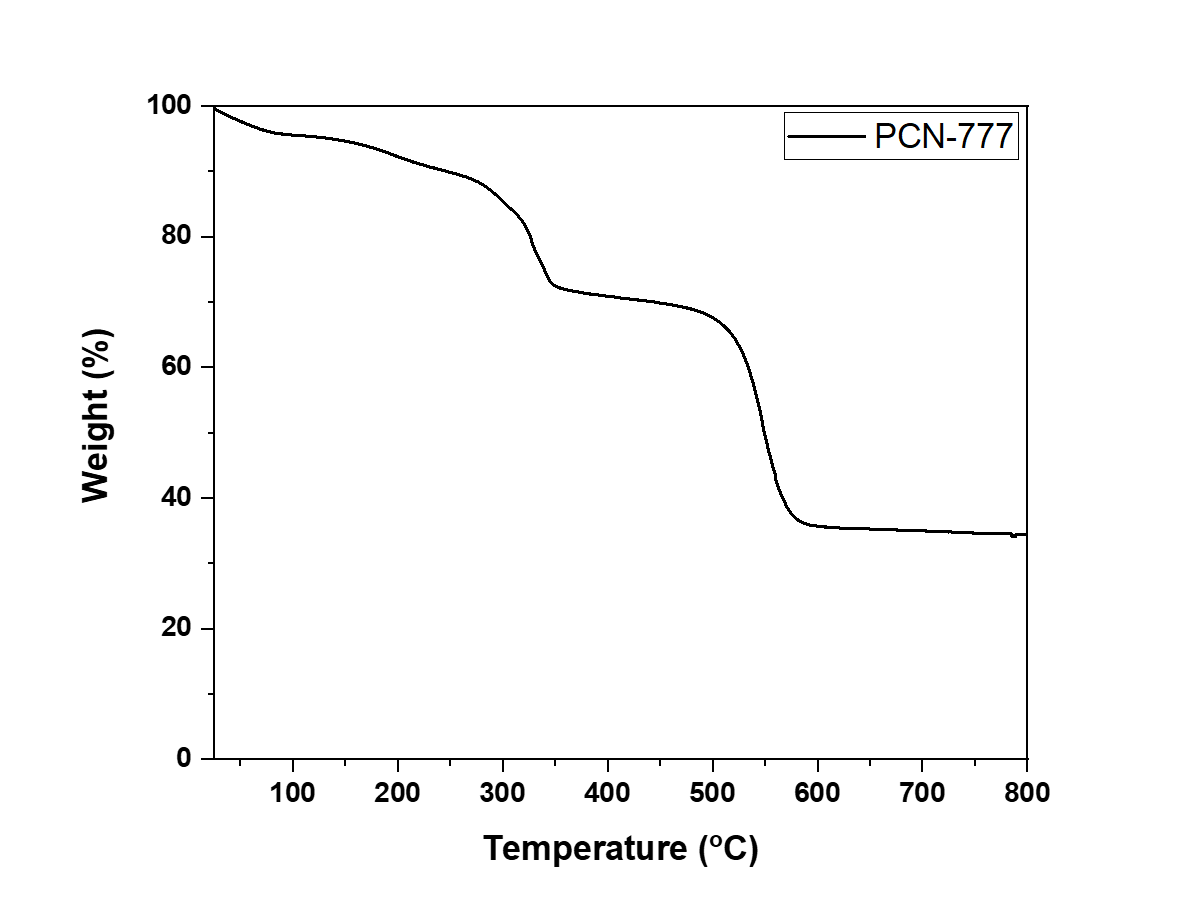
\includegraphics[width=0.8\textwidth]{pcn777_tga.png}
    \caption{%
        Thermogravimetric curve recorded on as-synthesised PCN-777.
    }\label{fig:tga}
\end{figure}

\begin{figure}[H]
    \centering
    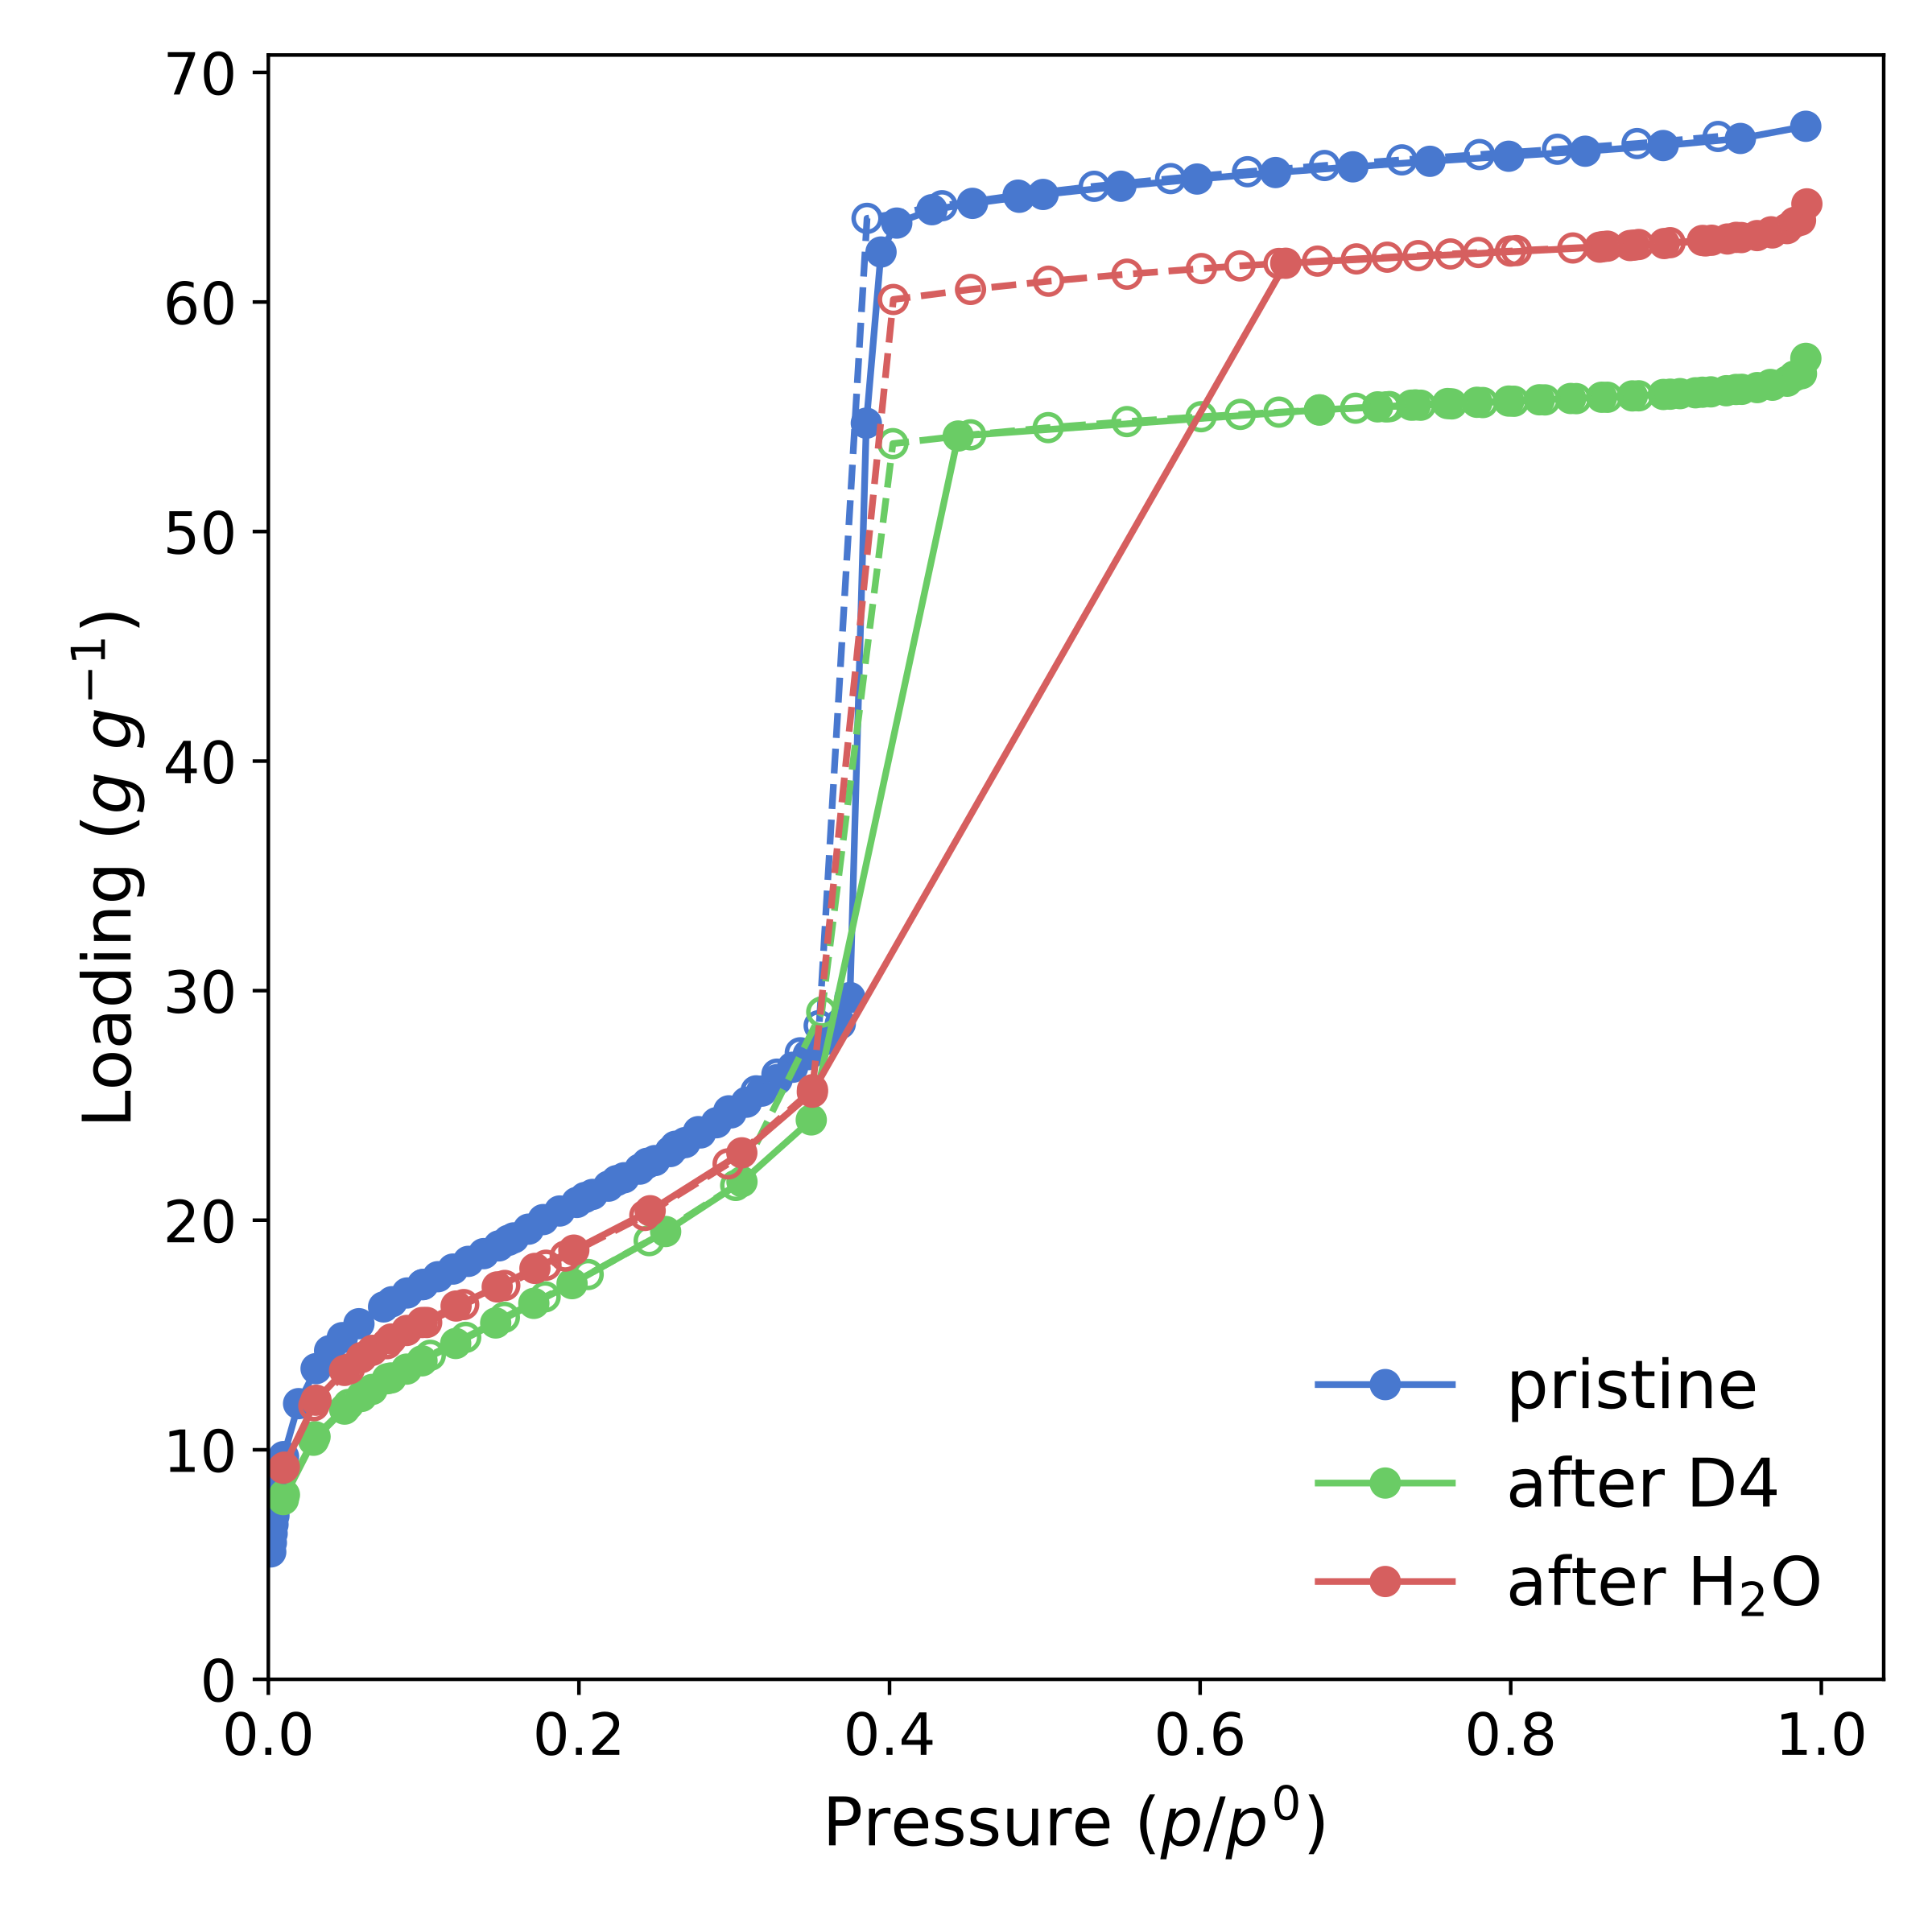
\includegraphics[width=0.6\textwidth]{n2-phys}
    \caption{%
        Nitrogen sorption isotherms at 77 K for the pristine
        PCN-777, alongside those measured on samples after D4 and water
        sorption.
    }\label{fig:n2-phys}
\end{figure}


\begin{figure}[H]
    \centering
    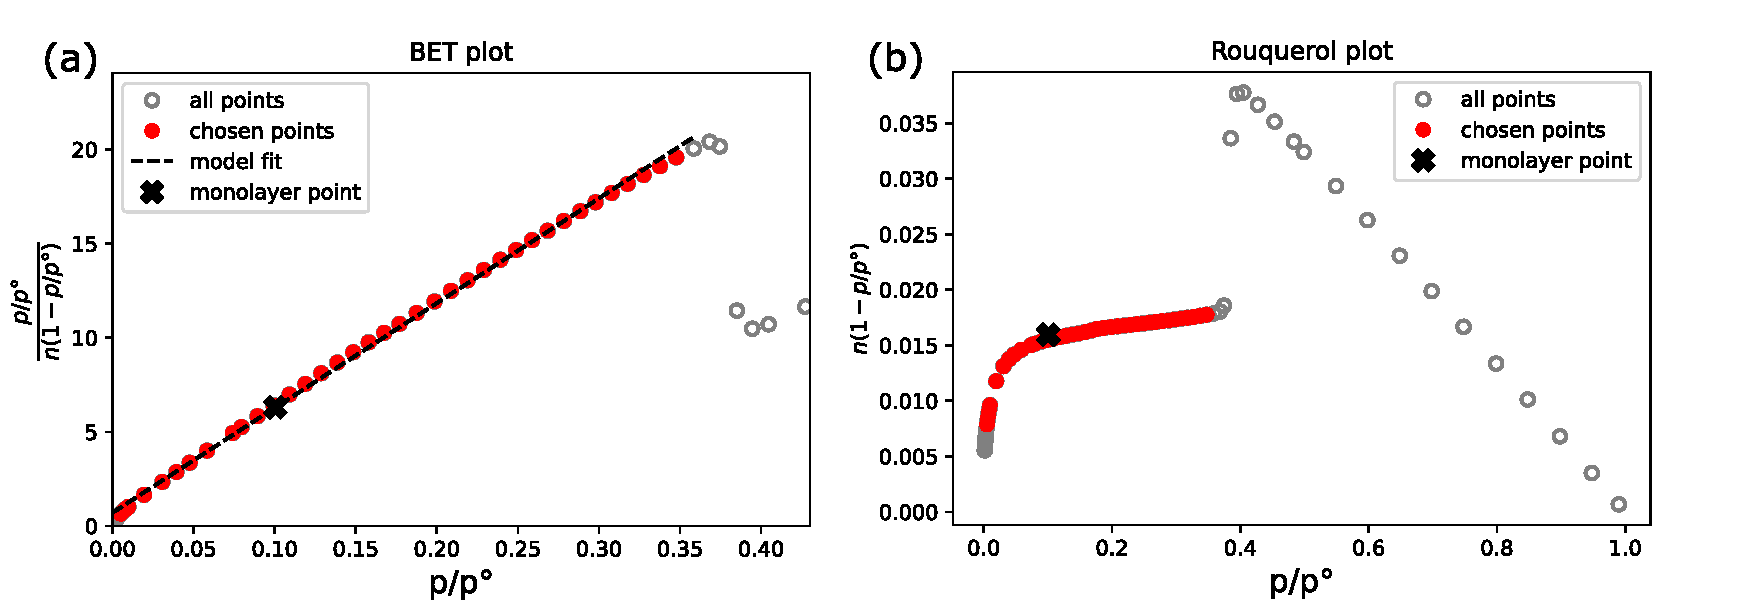
\includegraphics[width=0.8\textwidth]{n2-analysis}
    \caption{%
        BET and Rouquerol plots displaying selection of applicable
        isotherm points for the pristine PCN-777 isotherm.
    }\label{fig:n2-analysis}
\end{figure}

\pagebreak


\section{D4 sorption experiments}\label{d4-sorption-experiments}

\subsection{D4 benchmarking with known MOFs}\label{d4-benchmarking-with-known-mofs}

Isotherms were recorded on benchmark materials MIL-101(Cr) and DUT-4 using the
same methodology detailed in the main manuscript.

\begin{figure}[H]
    \centering
    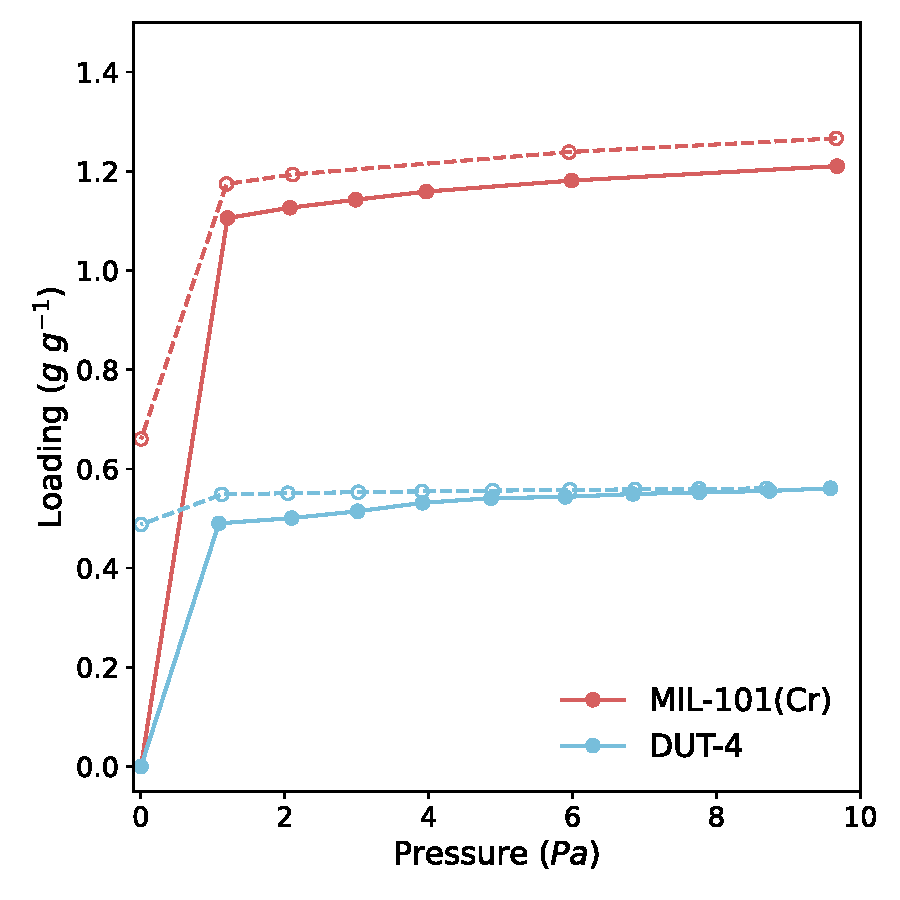
\includegraphics[width=0.5\textwidth]{benchmark-d4}
    \caption{%
        D4 isotherms recorded on samples of MIL-101(Cr) (red) and
        DUT-4 (blue), used to validate our computational methodology for
        predicting total D4 capacity. Note the different desorption behavior
        (open symbols) of the two materials under secondary vacuum: partial
        desorption for MIL-101(Cr) and no desorption for DUT-4.
    }\label{fig:d4-benchmark}
\end{figure}

\subsection{Isosteric heat of sorption of D4}\label{isosteric-heat-of-sorption-of-d4}

A further isotherm was recorded at \SI{313}{\kelvin} (\SI{40}{\degreeCelsius})
to allow for the calculation of the isosteric heat of adsorption through the
Clausius-Clapeyron equation, as depicted in \cref{fig:isosteric-enth}.

\begin{figure}[H]
    \centering
    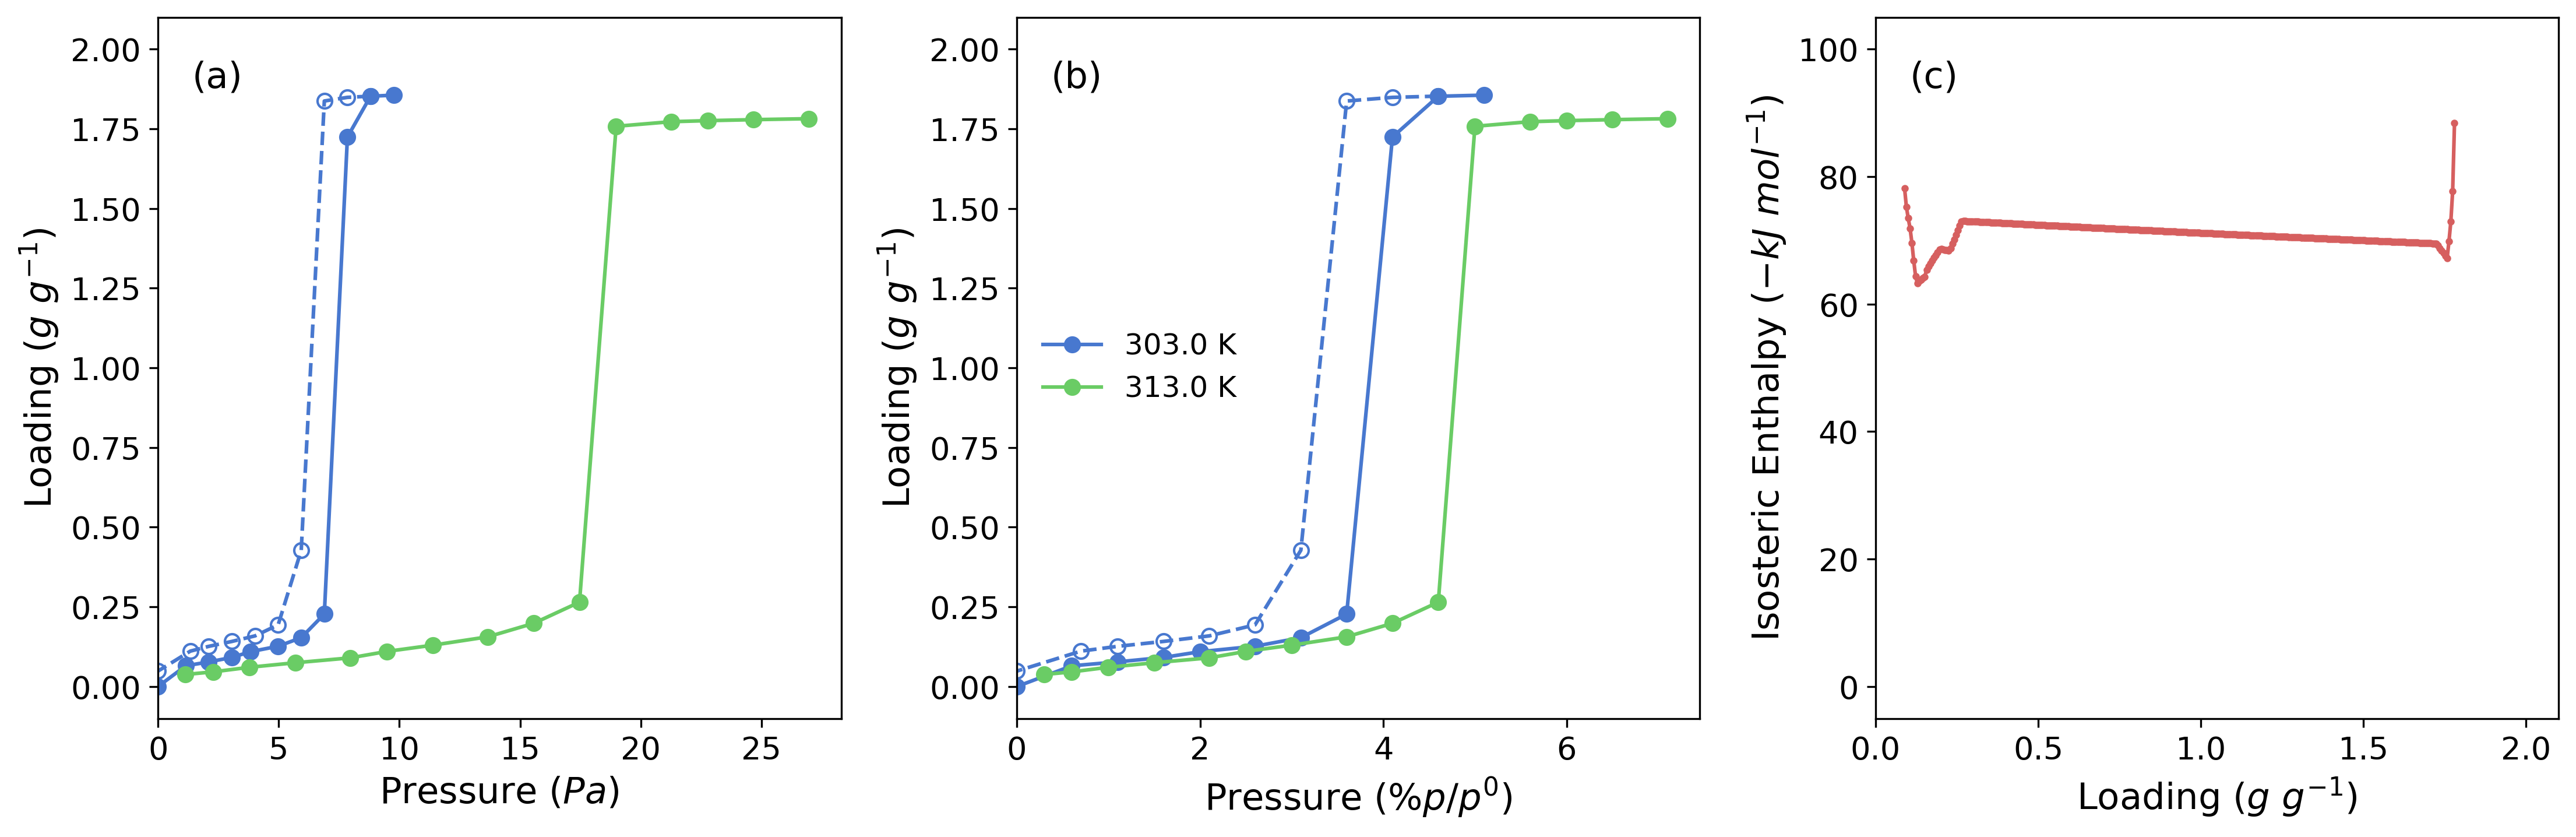
\includegraphics[width=\textwidth]{isosteric-enth}
    \caption{%
        D4 sorption isotherms on PCN-777 recorded at 303 K (blue)
        and at 313 K (green) in an absolute (a) and relative (b) pressure scale.
        (c) The calculated isosteric heat of adsorption as a function of D4
        uptake.
    }\label{fig:isosteric-enth}
\end{figure}
